\section{Tutorial -- ALAMO}
\label{sec.surrogate.alamo}
This tutorial focuses on the use of the ALAMO tool for building algebraic surrogate models. ALAMO builds simplified algebraic models, which are particularly well suited for rigorous equation oriented optimization. To keep the execution of this tutorial fast, a toy problem is used. In this case study the flowsheet calculations and sample generation are done within FOQUS, alternatively, the user can provide a simulation model such as: Excel, Aspen plus, Aspen custom modeler, etc. 

Note: Before starting this tutorial the ALAMO product must be downloaded from the products page on the CCSI website. The path for the ALAMO executable file must be set in FOQUS settings (see Section \ref{section.settings}).

\subsection{Flowsheet Setup}

\begin{enumerate}
	\item Open FOQUS.
	\item Name the session ``Surrogate\_Tutorial\_1'' (Figure \ref{fig.tut.sur.session}).
\end{enumerate}

\begin{figure}[H]
	\begin{center}
		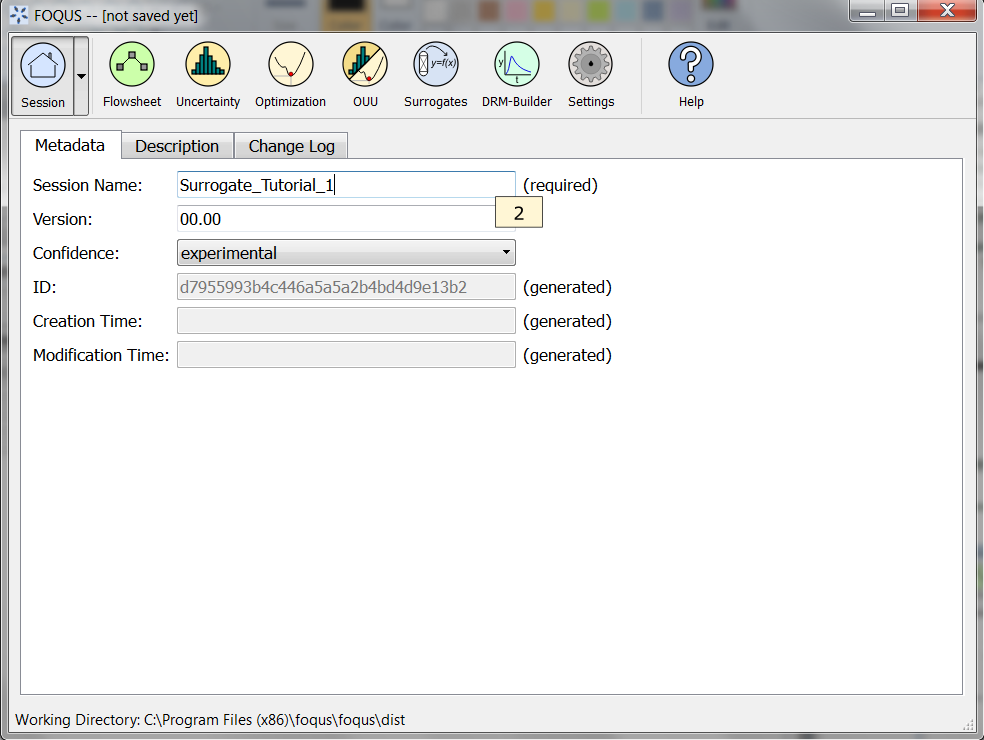
\includegraphics[scale=0.55]{Chapt_surrogates/figs/session1}
		\caption{Session Set Up}
		\label{fig.tut.sur.session}
	\end{center}
\end{figure}

\begin{enumerate}
	\setcounter{enumi}{2}
	\item Navigate to the Flowsheet Editor (Figure \ref{fig.tut.sur.flowsheet}).
	\item Add a Flowsheet Node named ``eq.''
	\item Display the Node Editor by clicking the \textbf{\underline{Node Editor}} toggle button.
\end{enumerate}
\begin{figure}[H]
	\begin{center}
		\includegraphics[scale=0.55]{Chapt_surrogates/figs/flowsheet}
		\caption{Flowsheet Setup}
		\label{fig.tut.sur.flowsheet}
	\end{center}
\end{figure}
The \textbf{\underline{Node Editor}} displays (Figure \ref{fig.tut.sur.nodeEdit.Input}).  The first step to setting up the node for this problem is to add input and output variables to the node.
%Does more detail need added to #9 below since the figure shows x1 and x2 in the Input Variables menu. Does the user need to know to click on Output Variables to open the Output Variables screen, then enter z1 and z2 under the Name column?
\begin{enumerate}
	\setcounter{enumi}{5}
	\item If the input variables table is not displayed as shown in Figure \ref{fig.tut.sur.nodeEdit.Input}, click the \textbf{\underline{Variables}} tab and then click the \textbf{\underline{Input Variables}} toolbox section.
	\item Add the variables ``x1'' and ``x2'' by clicking the \textbf{\underline{Add}} icon (+) above the input table.
	\item Edit the \textbf{\underline{Min/Max}} value for both variables to be ``-10.0'' and ``10.0.''
	\item Add two output variables ``z1'' and ``z2.''
\end{enumerate}
\begin{figure}[H]
	\begin{center}
		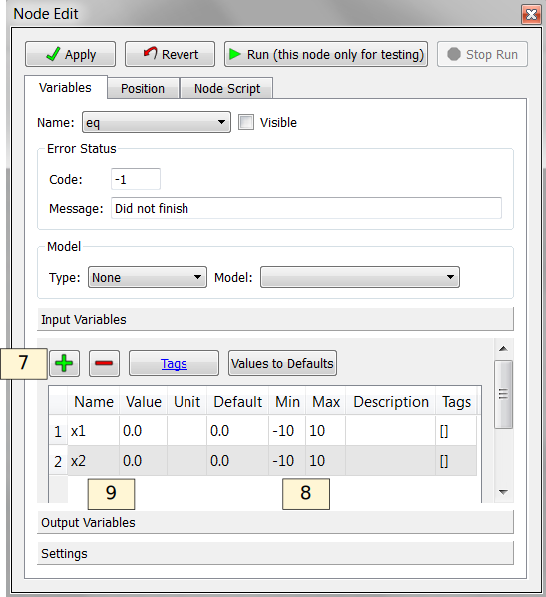
\includegraphics[scale=0.55]{Chapt_surrogates/figs/nodeInput}
		\caption{Node Variables}
		\label{fig.tut.sur.nodeEdit.Input}
	\end{center}
\end{figure}
To keep the execution time short, the node will not be assigned to a simulation model and calculations are performed directly in FOQUS.  
\begin{enumerate}
	\setcounter{enumi}{9}
	\item Click on the \textbf{\underline{Node Script}} tab in the Node Editor to enter the test equation (this step replaces the use of a simulator).
	\item Enter the following equations (Figure \ref{fig.tut.sur.nodeEdit.eq}):
	\begin{verbatim}
		f["z1"] = x["x1"] + x["x2"]
		f["z2"] = x["x1"]**2 + x["x2"]**2
	\end{verbatim}
	The node script calculations are written in Python. The dictionary ``f'' stores output values while the dictionary ``x'' stores input values.

\begin{figure}[H]
	\begin{center}
		\includegraphics[scale=0.55]{Chapt_surrogates/figs/nodeEq}
		\caption{Node Script}
		\label{fig.tut.sur.nodeEdit.eq}
	\end{center}
\end{figure}

	\item Test the model by running the flowsheet with the value ``2'' for ``x1'' and ``x2.'' After running, the output variables should have the values ``4.0'' for ``z1'' and ``8.0'' for ``z2.''
\end{enumerate}


\subsection{Creating Initial Samples}

There are two ways to start an ALAMO run: (1) generate a set of initial data, (2) use ALAMO's adaptive sampling with no initial data and let ALAMO generates its own samples. Adaptive sampling can be used with initial data to generate more points if needed. In this case, initial data is provided and adaptive sampling is used.

\begin{enumerate}
	\setcounter{enumi}{12}
	\item Select the UQ tool by clicking on the \textbf{\underline{Uncertainty}} button on the Home window (Figure \ref{fig.tut.sur.new.uq.ens}).
	\item Click the \textbf{\underline{Add New}} button.
	\item The \textbf{\underline{Add New Ensemble - Model Selection}} dialog will appear. Click \textbf{\underline{OK}} to set up the sampling scheme.
\end{enumerate}
\begin{figure}[H]
	\begin{center}
		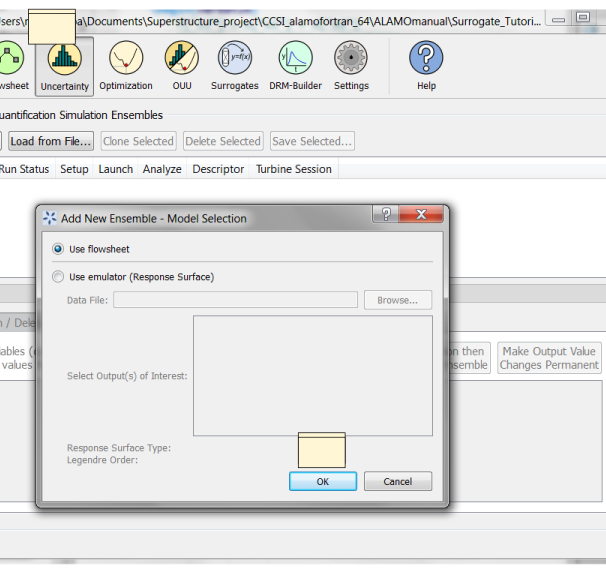
\includegraphics[scale=0.55]{Chapt_surrogates/figs/uqNewEns}
		\caption{Add a New Sample Ensemble}
		\label{fig.tut.sur.new.uq.ens}
	\end{center}
\end{figure}
\begin{enumerate}
	\setcounter{enumi}{15}
	\item The sample ensemble setup dialog displays (Figure \ref{fig.tut.sur.new.uq.sample1}).  Select \textbf{\underline{Choose sampling scheme}}. 
	\item Click the \textbf{\underline{All Variable}} button.
	\item Select the \textbf{\underline{Sampling scheme}} tab.
\end{enumerate}
\begin{figure}[H]
	\begin{center}
		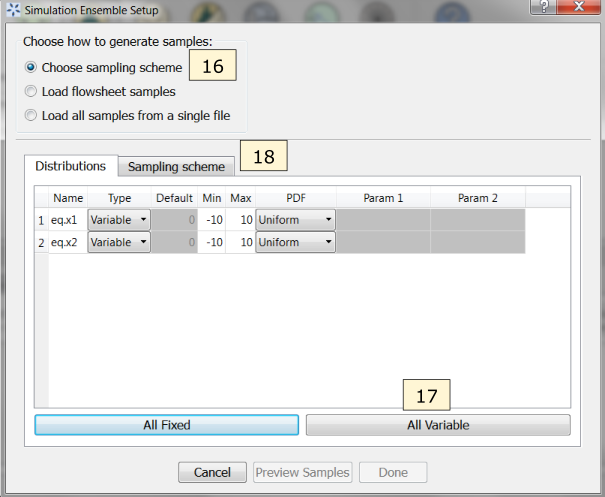
\includegraphics[scale=0.55]{Chapt_surrogates/figs/uqSample1}
		\caption{Sample Distributions}
		\label{fig.tut.sur.new.uq.sample1}
	\end{center}
\end{figure}
\begin{enumerate}
	\setcounter{enumi}{18}
	\item The \textbf{\underline{Sampling schem}e} dialog should display (Figure \ref{fig.tut.sur.new.uq.sample2}). Select ``Latin Hypercube'' from the list.
	\item Set the \textbf{\underline{\# of samples}} to ``10.''
	\item Click \textbf{\underline{Generate Samples}}.
	\item Click \textbf{\underline{Done}}.
\end{enumerate}
\begin{figure}[H]
	\begin{center}
		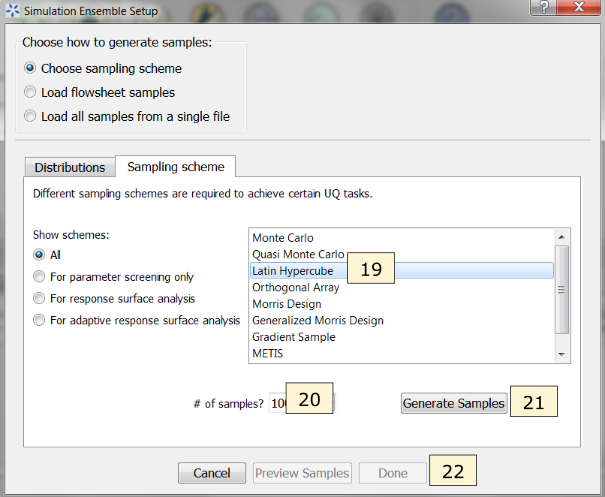
\includegraphics[scale=0.55]{Chapt_surrogates/figs/uqSample2}
		\caption{Sample Methods}
		\label{fig.tut.sur.new.uq.sample2}
	\end{center}
\end{figure}
\begin{enumerate}
\setcounter{enumi}{22}
\item Once the samples have been generated a new sample ensemble displays in the UQ tool window (Figure \ref{fig.tut.sur.new.uq.sample3}).  Click \textbf{\underline{Launch}} to run and generate the samples.
\end{enumerate}
\begin{figure}[H]
	\begin{center}
		\includegraphics[scale=0.55]{Chapt_surrogates/figs/uqSample3}
		\caption{Run Samples}
		\label{fig.tut.sur.new.uq.sample3}
	\end{center}
\end{figure}

\subsection{Data Selection}

Initial and validation data can be specified by creating filters that specify subsets of flowsheet data. In this tutorial only initial data will be used. A filter must be created to separate the results of the single test run from the UQ samples.

\begin{enumerate}
	\setcounter{enumi}{23}
	\item Click on the \textbf{\underline{Surrogates}} button from the Home window. The surrogate tool displays \ref{fig.tut.sur.data}.
	\item Select ``ALAMO'' from the \textbf{\underline{Tool}} drop-down list.
	\item Click \textbf{\underline{Edit Filters}} in the \textbf{\underline{Flowsheet Results}} section to create a filter.
\end{enumerate} 
\begin{figure}[H]
	\begin{center}
		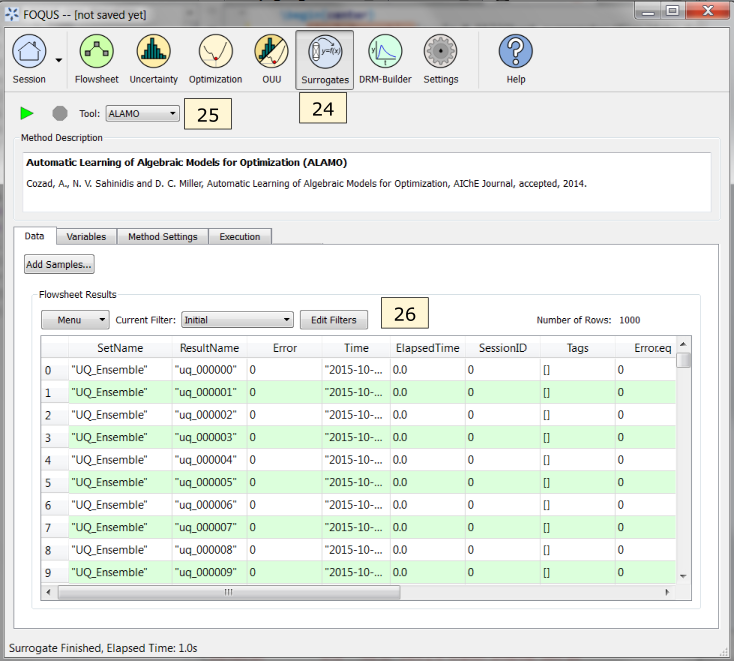
\includegraphics[scale=0.55]{Chapt_surrogates/figs/data}
		\caption{Surrogate Data}
		\label{fig.tut.sur.data}
	\end{center}
\end{figure}

\begin{enumerate}
	\setcounter{enumi}{26}
	\item Figure \ref{fig.tut.sur.dataFilter} displays the Data Filter Editor. 
	\item Add the filter for initial data.
	\begin{enumerate}
		\item Click \bu{New Filter}, and enter ``Initial'' as the filter name.
		\item Click \bu{Add Rule}.
		\item In the ``Term 1'' column enter: set (no quotes).
		\item In the ``Term 2'' column enter: ``UQ\_Ensemble'' (with quotes).
		\item In the ``Operator'' column select ``=.''	
	\end{enumerate}
	\item Click \textbf{\underline{Done}}.
\end{enumerate}
\begin{figure}[H]
	\begin{center}
		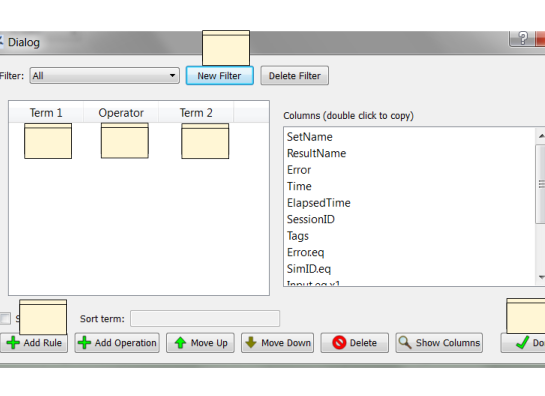
\includegraphics[scale=0.55]{Chapt_surrogates/figs/dataFilter}
		\caption{Data Filter Dialog}
		\label{fig.tut.sur.dataFilter}
	\end{center}
\end{figure}

\subsection{Variable Selection}
In this section, input and output variables need to be selected. Generally, any input variables that vary in the data set should be selected. However, in some cases, variables may be found to have no, or very little, effect on the outputs. Only the output variables of interest need to be selected. Note: Each output is independent from each other and for the model building, selecting one output is the same as selecting more.

\begin{enumerate}
	\setcounter{enumi}{29}
	\item Select the \textbf{\underline{Variable}s} tab (Figure \ref{fig.tut.sur.vaiables}).
	\item Select the checkbox for both input variables.
	\item Select the checkbox for both output variables.
\end{enumerate}
\begin{figure}[H]
	\begin{center}
		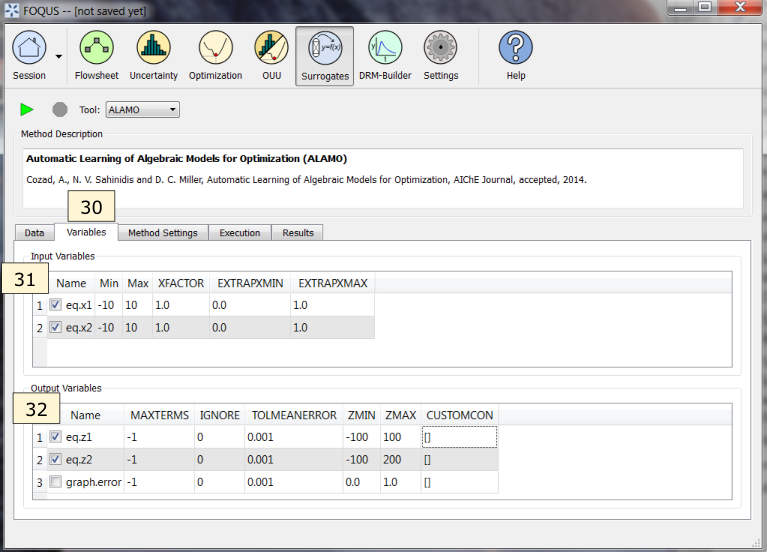
\includegraphics[scale=0.55]{Chapt_surrogates/figs/variables}
		\caption{Variable Selection}
		\label{fig.tut.sur.vaiables}
	\end{center}
\end{figure}

\subsection{Method Settings}
\label{tutorial.alamo.methodsettings}
The most important feature to generate "good" algebraic models is to configure the settings accordingly to the problem to be solved.  Each setting has a good description in FOQUS. The JSON parser is used to read method settings values. Strings must be contained in quotes. Lists have the following format: [element 1, element 2].

\begin{enumerate}
	\setcounter{enumi}{32}
	\item Click on the \textbf{\underline{Method Settings}} tab (see Figure \ref{fig.alamo.method.settigs}).
	\item Set the \textbf{\underline{FOQUS Model (for UQ)}} to ``ALAMO\_tutorial\_UQ.py.'' 
	\item Set the \textbf{\underline{FOQUS Model (for Flowsheet)}} to ``ALAMO\_tutorial\_FS.py''
	\item Set \textbf{\underline{Initial Data Filter}} to ``Initial.''
	\item Set \textbf{\underline{SAMPLER}} to select the adaptive sampling method: ``None'' ``Random'' or ``SNOBFIT.'' Use ``None'' in this tutorial.
	\item Set \textbf{\underline{MONOMIALPOWER}} to select the single variable term powers to [1,2,3].
	\item Set \textbf{\underline{MULTI2POWER}} to select the two variable term powers to [1].
	\item Select functions to be considered as basis functions (\textbf{\underline{EXPFCNS}}, \textbf{\underline{LOGFCNS}}, \textbf{\underline{SINFCNS}}, \textbf{\underline{COSFCNS}}).
	\item Leave the rest of settings as default (see Table \ref{tutorial.alamo.table}).
	\item Save this FOQUS session for use in the ACOSSO and BSS-ANOVA tutorials.
\end{enumerate}
\begin{figure}[H]
	\begin{center}
		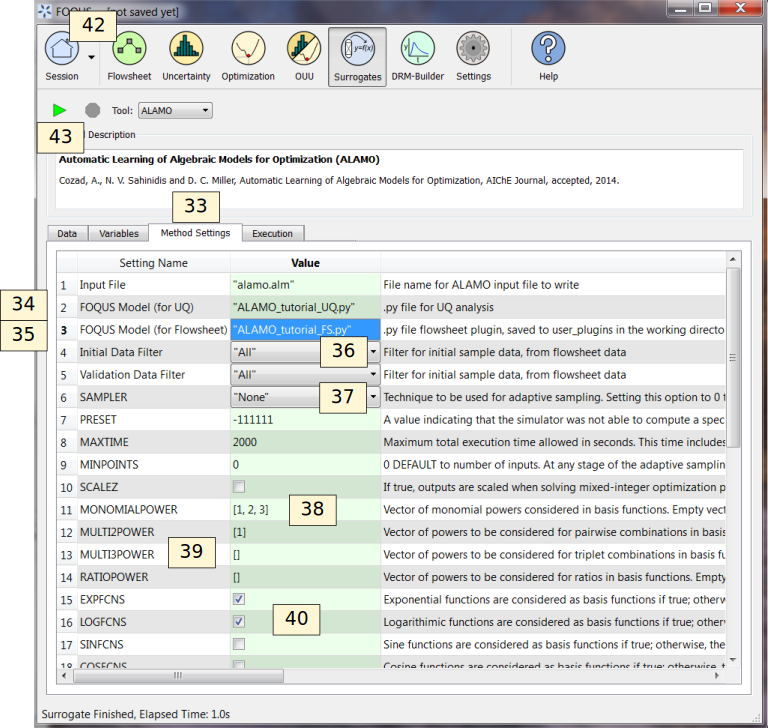
\includegraphics[scale=0.55]{Chapt_surrogates/figs/alamo_settings}
		\caption{ALAMO Method Settings}
		\label{fig.alamo.method.settigs}
	\end{center}
\end{figure}

\subsection{Execution}

\begin{enumerate}
	\setcounter{enumi}{42}
	\item Click the \bu{Run} icon at the top of the window.
	\item The ALAMO \bu{Execution} tab starts displaying execution file path, sub-directories, input files, and output files.
\begin{enumerate}
	\item ALAMO version.
	\item License Information.
	\item Step 0 displays the data set to be used by ALAMO.
	\item Step 1 displays the modeler used by ALAMO to generate the algebraic model.
	\item Once the surrogate model has finished, the equations are displayed in the execution window. It may be necessary to scroll up a little. The result is shown in Figure \ref{fig.alamo.res}.
	\item Finally, the statistics display the quality metrics of the models generated.
\end{enumerate}
\end{enumerate}

\begin{figure}[H]
	\begin{center}
		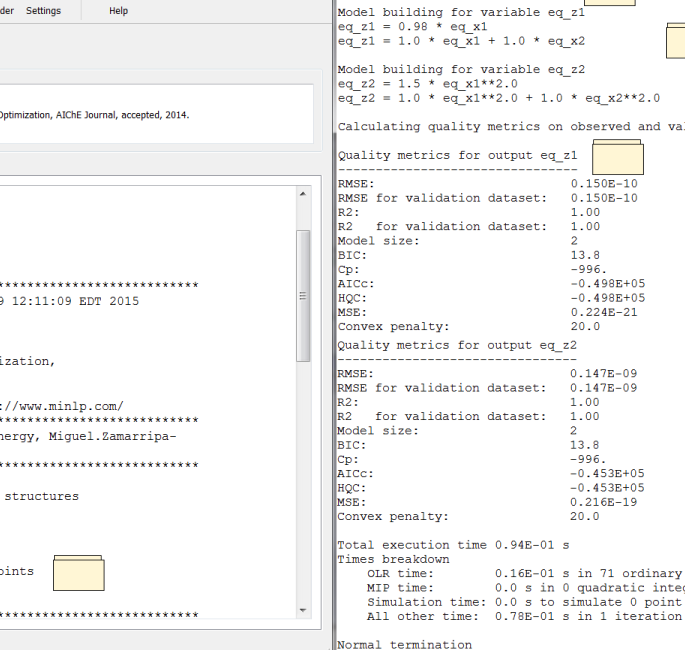
\includegraphics[scale=0.4]{Chapt_surrogates/figs/alamo_exec}
		\caption{ALAMO Execution}
		\label{fig.alamo.res}
	\end{center}
\end{figure}

\subsection{Results}
	The results are exported as a PSUADE driver file that can be used perform UQ analysis of the models, and a FOQUS Python plugin model that allows it to be used in a FOQUS flowsheet. The equations can also be viewed in the results section.
	
	See tutorial Section \ref{tutorial.surrogate.uq} and \ref{tutorial.surrogate.fs} for information about analyzing the model with the UQ tools or running the model on the flowsheet.
	
	As mentioned in section \ref{tutorial.alamo.methodsettings} the method settings are very important. A brief description and hints are included in Table \ref{tutorial.alamo.table}.

\begin{center}

\begin{longtable}{|p{.30\textwidth}|p{.70\textwidth} |}
\caption{ALAMO Method Settings}
\label{tutorial.alamo.table} \\

		\hline
			\textbf{Method Settings} & \textbf{Description} \\		\hline
			Initial Data Filter & Filter to be applied to the initial data set. Data filters help the user to generate models based on specific data for each variable.  \\	\hline
			Validation Data filter & Data set used to compute model errors at the validation phase. The number of data points in a preexisting validation data set can be specified by the user.\\	\hline
			SAMPLER & Adaptative sampling method to be used. Options: "None", "Random" and "SNOBFIT". Adaptive sampling method to be used by ALAMO when more sampling points are needed by the model. If \bu{Random} is used a simulator must be provided by the user. If \bu{SNOBFIT} is used a simulator must be provided by the user and MATLAB must be installed.\\	\hline
			MAXTIME& Maximum execution time in seconds. This time includes all the steps on the algorithm, if simulations are needed they run in this time.\\	\hline
			MINPOINTS& Convergence is assessed only if the simulator is able to compute the output variables for at least MINPOINTS of the data set. A reduced number of MINPOINTS may reduce the computational time to get a model, but also reduces the accuracy of the model. MINPOINTS must be a positive integer. \\ \hline
			PRESET&Value to be used if the simulator fails. This value must be carefully chosen to be an otherwise not realizable value for the output variables.\\ \hline
			MONOMIALPOWERS &  Vector of monomial powers to be considered as basis functions, use empty vector for none []. Exponential terms allowed in the algebraic model.  i.e., if selecting [1,2] the model considers x1 and x1**2 as basis functions. \\ \hline
			MULTI2POWER & Vector of pairwise combination of powers to be considered as basis functions. Pairwise combination of powers allowed in the algebraic model. i.e., [1,2] allows terms like x1*x2 in the algebraic model.\\ \hline
			MULTI3POWER & Vector of three variables combinations of powers to be considered as basis functions. \\ \hline
			\raggedright{EXPFCNS, LOGFCNS, SINFCNS, COSFCNS functions}& Use or not of exp, log, sin, and cos functions as basis functions in the model. \\ \hline
			RATIOPOWER& Vector of ratio combinations of powers to be considered in the basis functions. Ratio combinations of powers are [empty as default].\\ \hline
			Radial Basis Functions& Radial basis functions centered around the data set provided by the user. These functions are Gaussian and are deactivated if their textual representation requires more than 128 characters (in the case of too many input variables and/or datapoints). \\ \hline
			RBF parameter&Constant penalty used in the Gaussian radial basis functions.  \\ \hline
			Modeler & Fitness metric to be used for model building. Options: BIC (Bayesian Information Criterion), Mallow's Cp, AICc (Corrected Akaike's Information Criterio), HQC (Hannan-Quinn Information Criterion), MSE (Mean Square Error), and Convex Penalty. \\ \hline
			ConvPen& Convex penalty term. Used if Convex Penalty is selected. \\ \hline
			Regularizer & Regularization method is used to reduce the number of potential basis functions before the optimization.\\ \hline 
			Tolrelmetric & Convergence tolerance for the chosen fitness metric is needed to terminate the algorithm. \\ \hline
			ScaleZ&If used, the variables are scaled prior to the optimization problem is solved. The problem is solved using a mathematical programming solver. Usually, scaling the variables may help the optimization procedure.\\ \hline
			GAMS&GAMS is the software used to solve the optimization problems. The executable path is expected or the user must declare GAMS.exe in the environment path.\\ \hline
			GAMS Solver&Solver to be used by GAMS to solve the optimization problems. Mixed integer quadratic programming solver is expected like BARON (other solvers can be used).\\ \hline
			MIPOPTCR & Relative convergence tolerance for the optimization problems solved in GAMS. The optimization problem is solved when the optcr is reached. 5 to 1 \% is expected (0.005 to 0.001).\\ \hline
			MIPOPTCA & Absolute convergence tolerance for mixed-integer optimization problems. This must be a nonnegative scalar. \\ \hline
			Linear error & If true, a linear objective function is used when solving the mixed integer optimization problems; otherwise, a quadratic objective function is used. \\ \hline
			\raggedright{Constraint Regression (CONREG)} & Specify whether constraint regression is used or not, if true bounds on output variables are enforced. \\ \hline
			CRNCUSTOM & If true, Custom constraints are entered in the Variable tab.\\ \hline
			CRNINITIAL& Number of random bounding points at which constraints are sampled initially (must be a nonnegative integer). \\ \hline
			CRNMAXITER & Maximum allowed constrained regressions iterations. Constraints are enforced on additional points during each iteration (must be positive integer). \\ \hline
			CRNVIOL & Number of bounding points added per round per bound in each iteration (must be positive integer). \\ \hline
			CRNTRIALS&Number of random trial bounding points per round of constrained regression (must be a positive integer). \\ \hline
			CUSTOMBAS&A list of user-supplied custom basis functions can be provided by the user. The parser is not case sensitive and allows for any Fortran functional expression in terms of the XLABELS (symbol \^{} may be used to denote power). \\ \hline
			
%		\end{tabularx}
%	\end{center}

\end{longtable}	
\end{center}	
